
% \section{Deployment View}

% \subsection{Introduction and Architecture}
% \textbf{Architecture Overview} Hệ thống IoT-SPMS sử dụng kiến trúc web nhiều tầng (Multi-tier Architecture) nhằm đảm bảo khả năng mở rộng, dễ bảo trì và hỗ trợ tích hợp linh hoạt với các thiết bị IoT trong bãi đỗ xe thông minh. Kiến trúc hệ thống bao gồm các tầng chính sau:
% \begin{itemize}
%     \item \textbf{Presentation Tier:} Giao diện người dùng, được xây dựng dưới dạng Single-Page Application (SPA) sử dụng React.js, hỗ trợ truy cập qua trình duyệt web và thiết bị di động.
%     \item \textbf{Application Tier:} Xử lý logic nghiệp vụ cốt lõi và quản lý luồng dữ liệu IoT, được triển khai dưới dạng REST API sử dụng Node.js/Express.js và tích hợp sẵn MQTT Broker.
%     \item \textbf{Data Tier:} Quản lý việc lưu trữ và truy xuất dữ liệu, bao gồm cơ sở dữ liệu PostgreSQL cho dữ liệu có cấu trúc, Redis cho bộ nhớ đệm và MinIO cho dữ liệu không cấu trúc.
%     \item \textbf{IoT Edge Layer:} Phụ trách thu thập dữ liệu từ các cảm biến hiện trường và điều khiển các thiết bị ngoại vi tại bãi xe.
% \end{itemize}

% \subsection{Deployment Architecture Diagram}
% \begin{figure}[H]
%     \centering
%     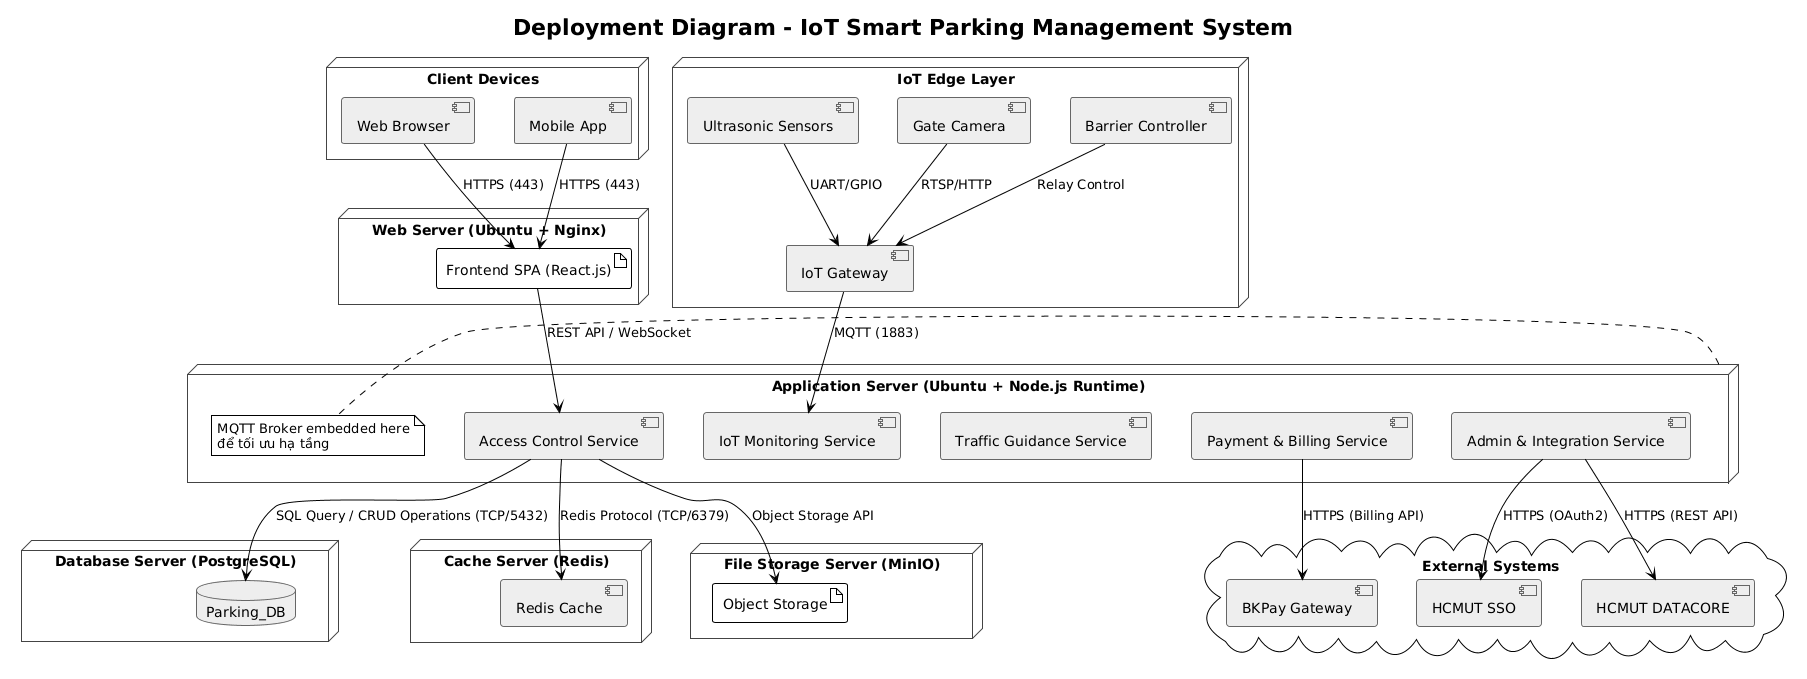
\includegraphics[width=1.0\textwidth]{pictures/deploymentdiagram.png}
%     \caption{The overall deployment architecture of the HCMUT Smart Parking Management System, illustrating the interaction between clients, servers, and edge IoT devices.}
%     \label{fig:deployment-architecture}
% \end{figure}

% \subsection{System Components and Servers}
% \textbf{System Components Overview} Hệ thống bao gồm 5 máy chủ chuyên dụng và tích hợp với 3 hệ thống ngoại vi cốt lõi của hạ tầng HCMUT để đảm bảo tính nhất quán dữ liệu và trải nghiệm người dùng liền mạch.
% \begin{itemize}
%     \item \textbf{Main Servers:}
%     \begin{enumerate}
%         \item Web Server (Nginx)
%         \item Application Server (Node.js/Express.js)
%         \item Database Server (PostgreSQL)
%         \item Cache Server (Redis)
%         \item File Storage Server (MinIO)
%     \end{enumerate}
%     \item \textbf{External Systems (HCMUT Infrastructure):}
%     \begin{enumerate}
%         \item HCMUT\_SSO (Dịch vụ xác thực tập trung)
%         \item HCMUT\_DATACORE (Hệ thống đồng bộ dữ liệu sinh viên/giảng viên)
%         \item BKPay Gateway (Cổng thanh toán nội bộ nhà trường)
%     \end{enumerate}
% \end{itemize}

% \subsection{Server Specifications}
% \textbf{Web Server (Nginx)} 
% \begin{itemize}
%     \item \textbf{OS:} Ubuntu Server 22.04 LTS
%     \item \textbf{Deployed Components:} Frontend Application (React.js production build) và các tài nguyên tĩnh (HTML, CSS, JS bundles).
%     \item \textbf{Responsibilities:} Cung cấp giao diện web cho người dùng, xử lý chứng chỉ bảo mật HTTPS và đóng vai trò Reverse Proxy điều phối các yêu cầu API đến Application Server.
% \end{itemize}

% \textbf{Application Server (Node.js / Express.js)} 
% \begin{itemize}
%     \item \textbf{OS:} Ubuntu Server 22.04 LTS
%     \item \textbf{Runtime:} Node.js 18.x LTS
%     \item \textbf{Deployed Components:} Backend REST API, được phân chia logic thành các phân hệ: Access Control, IoT Monitoring, Traffic Guidance và Payment \& Billing. Tích hợp sẵn \textbf{Embedded MQTT Broker} để quản lý thông điệp từ thiết bị.
%     \item \textbf{Responsibilities:} Thực thi toàn bộ logic nghiệp vụ, xử lý các API endpoints, kết nối với các dịch vụ dữ liệu và tích hợp với các hệ thống ngoại vi của HCMUT.
% \end{itemize}

% \textbf{Database Server (PostgreSQL)} 
% \begin{itemize}
%     \item \textbf{OS:} Ubuntu Server 22.04 LTS
%     \item \textbf{Software:} PostgreSQL 15
%     \item \textbf{Responsibilities:} Lưu trữ dữ liệu bền vững (phiên gửi xe, trạng thái ô đỗ), đảm bảo tính toàn vẹn dữ liệu. Hệ thống thực hiện chiến lược sao lưu dữ liệu định kỳ hàng ngày.
% \end{itemize}

% \textbf{Cache Server (Redis)} 
% \begin{itemize}
%     \item \textbf{OS:} Ubuntu Server 22.04 LTS
%     \item \textbf{Software:} Redis 7.x
%     \item \textbf{Responsibilities:} Lưu trữ đệm các dữ liệu truy cập thường xuyên như trạng thái chỗ trống thời gian thực để tối ưu tốc độ truy xuất.
% \end{itemize}

% \textbf{File Storage Server (MinIO)} 
% \begin{itemize}
%     \item \textbf{OS:} Ubuntu Server 22.04 LTS
%     \item \textbf{Software:} MinIO (S3-compatible object storage)
%     \item \textbf{Responsibilities:} Lưu trữ dữ liệu không cấu trúc như hình ảnh nhận diện biển số từ camera và ảnh đại diện người dùng.
% \end{itemize}

% \textbf{IoT Edge Layer (Hạ tầng hiện trường)} 
% \begin{itemize}
%     \item \textbf{Components:} IoT Gateway, Ultrasonic Sensors, Gate Camera, Barrier Controller.
%     \item \textbf{Responsibilities:} Thu thập trạng thái thực tế từ các ô đỗ xe và truyền tải dữ liệu về trung tâm thông qua giao thức MQTT.
% \end{itemize}

% \subsection{External System Integration}
% \noindent \textbf{HCMUT\_SSO (Single Sign-On)} Việc tích hợp thực hiện qua OAuth 2.0. Khi đăng nhập, hệ thống chuyển hướng đến cổng HCMUT\_SSO để xác thực, đảm bảo an toàn và đồng bộ với tài khoản nhà trường.

% \medskip
% \noindent \textbf{HCMUT\_DATACORE} Hệ thống truy vấn DATACORE qua API bảo mật để xác định vai trò người dùng và thông tin phương tiện, từ đó áp dụng các chính sách giá và quyền truy cập bãi xe tương ứng.

% \medskip
% \noindent \textbf{BKPay Gateway} Tích hợp qua Billing API để tự động hóa quy trình thanh toán phí gửi xe, khởi tạo giao dịch và nhận phản hồi thời gian thực để điều khiển barrier tại cổng.

% \subsection{Communication Protocols and Security}
% \textbf{Protocol Summary} Bảng dưới đây tóm tắt các giao thức truyền thông chính được sử dụng trong hệ thống:
% \begin{table}[H]
%     \centering
%     \caption{Summary of key communication protocols within the IoT-SPMS system.}
%     \label{tab:protocols}
%     \begin{tabular}{|l|l|l|l|}
%         \hline
%         \textbf{From} & \textbf{To} & \textbf{Protocol (Port)} & \textbf{Purpose} \\ \hline
%         Client Browser & Web Server & HTTPS (443) & Secure web access \\ \hline
%         IoT Gateway & App Server & MQTT (1883) & Sensor data transmission \\ \hline
%         App Server & Database & PostgreSQL (5432) & Data queries \\ \hline
%         App Server & Cache Server & Redis (6379) & Cache operations \\ \hline
%         App Server & External Systems & HTTPS (443) & Secure API integration \\ \hline
%     \end{tabular}
% \end{table}

% \noindent \textbf{Security Measures} Bảo mật được thực thi đa lớp: mã hóa HTTPS, băm mật khẩu bằng bcrypt, quản lý quyền bằng RBAC kết hợp JWT tokens, và thiết lập tường lửa giới hạn giao tiếp nội bộ giữa các server.

% \subsection{Scalability and Disaster Recovery}
% \noindent \textbf{Scalability} Kiến trúc hỗ trợ mở rộng chiều ngang cho tầng Web và App. Tầng dữ liệu có thể nâng cấp tài nguyên hoặc nhân bản. Giao thức MQTT giúp dễ dàng mở rộng số lượng cảm biến mà không ảnh hưởng hiệu năng trung tâm.

% \medskip
% \noindent \textbf{Disaster Recovery} Kế hoạch phục hồi bao gồm sao lưu ngoại vi hàng ngày, quản lý cấu hình qua phiên bản (Git). Mục tiêu RTO dưới 4 giờ.  Khi phát hiện mất kết nối thông qua việc gián đoạn tín hiệu Heartbeat, tầng IoT Edge sẽ tự động chuyển sang chế độ vận hành độc lập (Offline mode).
% \subsection{Technology Stack Overview} 
% Tóm tắt toàn bộ công nghệ cốt lõi của hệ thống IoT-SPMS:
% \begin{table}[H]
%     \centering
%     \caption{Summary of the primary technology stack for IoT-SPMS.}
%     \label{tab:tech-stack}
%     \begin{tabular}{|l|l|}
%         \hline
%         \textbf{Component} & \textbf{Technology} \\ \hline
%         Frontend & React.js 18.x, Tailwind CSS, Vite \\ \hline
%         Web Server & Nginx 1.24 \\ \hline
%         Backend & Node.js 18.x with Express.js 4.x \\ \hline
%         IoT Communication & MQTT Protocol, WebSockets \\ \hline
%         Database & PostgreSQL 15.x \\ \hline
%         Cache & Redis 7.x \\ \hline
%         File Storage & MinIO \\ \hline
%         IoT Hardware & ESP32 / Raspberry Pi, Ultrasonic Sensors \\ \hline
%         Operating System & Ubuntu Server 22.04 LTS (all servers) \\ \hline
%     \end{tabular}
% \end{table}

% \noindent \textbf{Justification of Stack Selection} Lựa chọn Node.js và MQTT đảm bảo xử lý hàng nghìn thông điệp từ cảm biến với độ trễ thấp, trong khi Ubuntu Server và PostgreSQL mang lại sự ổn định và bảo mật tối đa cho dữ liệu bãi xe.

 \section{Deployment View}
\subsection{Giới thiệu và Kiến trúc}
\textbf{Tổng quan kiến trúc} Hệ thống IoT-SPMS sử dụng kiến trúc web nhiều tầng (Multi-tier Architecture) nhằm đảm bảo khả năng mở rộng, dễ bảo trì và hỗ trợ tích hợp linh hoạt với các thiết bị IoT trong bãi đỗ xe thông minh. Kiến trúc hệ thống bao gồm các tầng chính sau:
\begin{itemize}
    \item \textbf{Presentation Tier:} Giao diện người dùng, được xây dựng dưới dạng Single-Page Application (SPA) sử dụng React.js, hỗ trợ truy cập qua trình duyệt web và thiết bị di động.
    \item \textbf{Application Tier:} Xử lý logic nghiệp vụ cốt lõi và quản lý luồng dữ liệu IoT, được triển khai dưới dạng REST API sử dụng Node.js/Express.js và tích hợp sẵn MQTT Broker.
    \item \textbf{Data Tier:} Quản lý việc lưu trữ và truy xuất dữ liệu, bao gồm cơ sở dữ liệu PostgreSQL cho dữ liệu có cấu trúc, Redis cho bộ nhớ đệm và MinIO cho dữ liệu không cấu trúc.
    \item \textbf{IoT Edge Layer:} Phụ trách thu thập dữ liệu từ các cảm biến hiện trường và điều khiển các thiết bị ngoại vi tại bãi xe.
\end{itemize}

\subsection{Sơ đồ Kiến trúc Triển khai}
\begin{figure}[H]
    \centering
    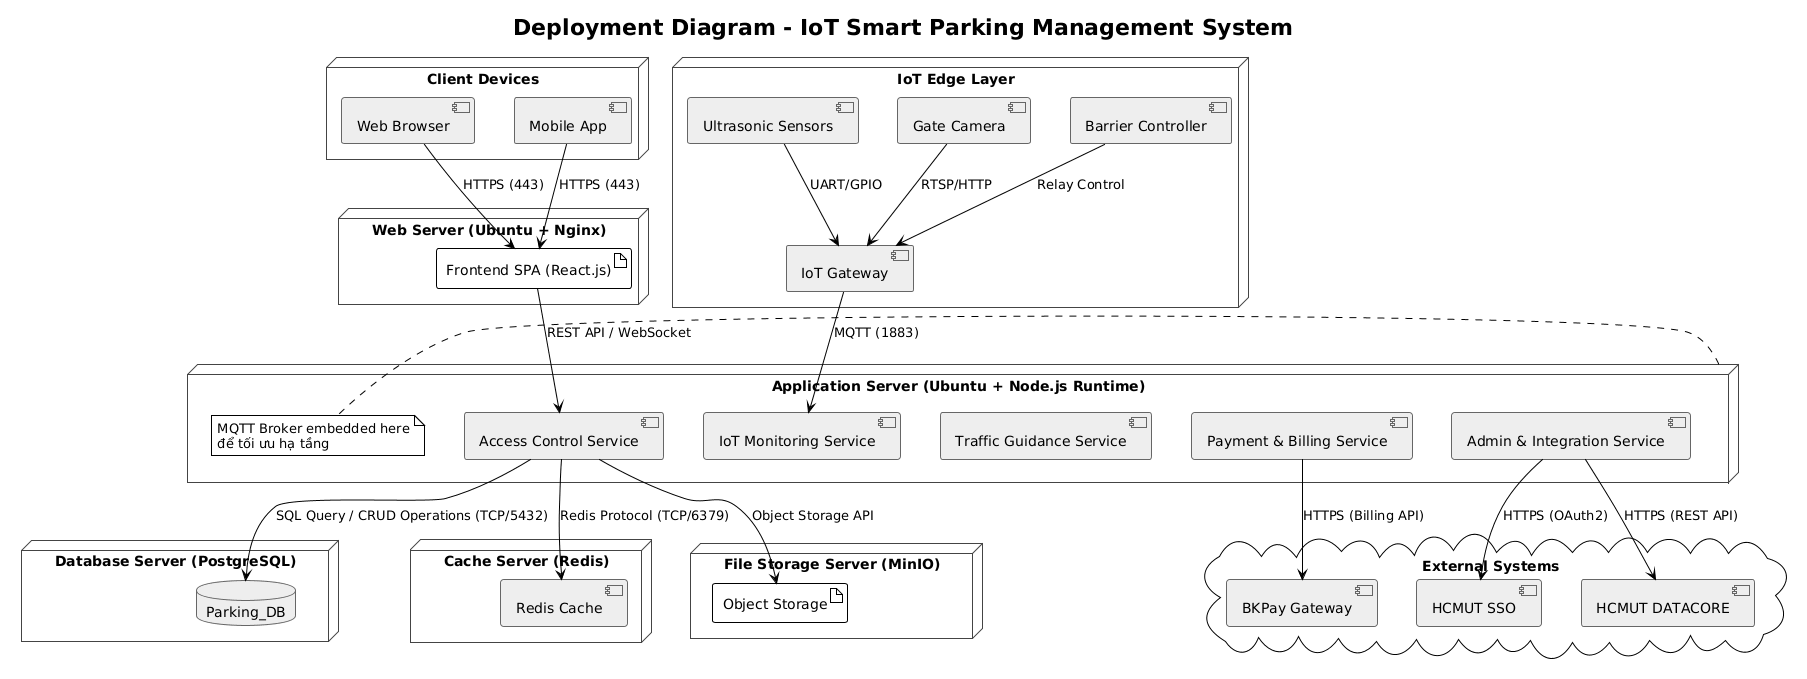
\includegraphics[width=1.0\textwidth]{pictures/deploymentdiagram.png}
    \caption{Kiến trúc triển khai tổng thể của Hệ thống Quản lý Bãi đỗ xe Thông minh HCMUT, minh họa sự tương tác giữa máy khách, máy chủ và các thiết bị IoT hiện trường.}
    \label{fig:deployment-architecture}
\end{figure}

\subsection{Thành phần Hệ thống và Máy chủ}
\textbf{Tổng quan Thành phần Hệ thống} Hệ thống bao gồm 5 máy chủ chuyên dụng và tích hợp với 3 hệ thống ngoại vi cốt lõi của hạ tầng HCMUT để đảm bảo tính nhất quán dữ liệu và trải nghiệm người dùng liền mạch.
\begin{itemize}
    \item \textbf{Máy chủ chính:}
    \begin{enumerate}
        \item Web Server (Nginx)
        \item Application Server (Node.js/Express.js)
        \item Database Server (PostgreSQL)
        \item Cache Server (Redis)
        \item File Storage Server (MinIO)
    \end{enumerate}
    \item \textbf{Hệ thống ngoại vi (Hạ tầng HCMUT):}
    \begin{enumerate}
        \item HCMUT\_SSO (Dịch vụ xác thực tập trung)
        \item HCMUT\_DATACORE (Hệ thống đồng bộ dữ liệu sinh viên/giảng viên)
        \item BKPay Gateway (Cổng thanh toán nội bộ nhà trường)
    \end{enumerate}
\end{itemize}

\subsection{Thông số kỹ thuật Máy chủ}
\textbf{Web Server (Nginx)} 
\begin{itemize}
    \item \textbf{Hệ điều hành:} Ubuntu Server 22.04 LTS
    \item \textbf{Thành phần triển khai:} Ứng dụng Frontend (React.js production build) và các tài nguyên tĩnh (HTML, CSS, JS bundles).
    \item \textbf{Trách nhiệm:} Cung cấp giao diện web cho người dùng, xử lý chứng chỉ bảo mật HTTPS và đóng vai trò Reverse Proxy điều phối các yêu cầu API đến Application Server.
\end{itemize}

\textbf{Application Server (Node.js / Express.js)} 
\begin{itemize}
    \item \textbf{Hệ điều hành:} Ubuntu Server 22.04 LTS
    \item \textbf{Runtime:} Node.js 18.x LTS
    \item \textbf{Thành phần triển khai:} Backend REST API, được phân chia logic thành các phân hệ: Access Control, IoT Monitoring, Traffic Guidance và Payment \& Billing. Tích hợp sẵn \textbf{Embedded MQTT Broker} để quản lý thông điệp từ thiết bị.
    \item \textbf{Trách nhiệm:} Thực thi toàn bộ logic nghiệp vụ, xử lý các API endpoints, kết nối với các dịch vụ dữ liệu và tích hợp với các hệ thống ngoại vi của HCMUT.
\end{itemize}

\textbf{Database Server (PostgreSQL)} 
\begin{itemize}
    \item \textbf{Hệ điều hành:} Ubuntu Server 22.04 LTS
    \item \textbf{Phần mềm:} PostgreSQL 15
    \item \textbf{Trách nhiệm:} Lưu trữ dữ liệu bền vững (phiên gửi xe, trạng thái ô đỗ), đảm bảo tính toàn vẹn dữ liệu. Hệ thống thực hiện chiến lược sao lưu dữ liệu định kỳ hàng ngày.
\end{itemize}

\textbf{Cache Server (Redis)} 
\begin{itemize}
    \item \textbf{Hệ điều hành:} Ubuntu Server 22.04 LTS
    \item \textbf{Phần mềm:} Redis 7.x
    \item \textbf{Trách nhiệm:} Lưu trữ đệm các dữ liệu truy cập thường xuyên như trạng thái chỗ trống thời gian thực để tối ưu tốc độ truy xuất.
\end{itemize}

\textbf{File Storage Server (MinIO)} 
\begin{itemize}
    \item \textbf{Hệ điều hành:} Ubuntu Server 22.04 LTS
    \item \textbf{Phần mềm:} MinIO (S3-compatible object storage)
    \item \textbf{Trách nhiệm:} Lưu trữ dữ liệu không cấu trúc như hình ảnh nhận diện biển số từ camera và ảnh đại diện người dùng.
\end{itemize}

\textbf{IoT Edge Layer (Hạ tầng hiện trường)} 
\begin{itemize}
    \item \textbf{Thành phần:} IoT Gateway, Ultrasonic Sensors, Gate Camera, Barrier Controller.
    \item \textbf{Trách nhiệm:} Thu thập trạng thái thực tế từ các ô đỗ xe và truyền tải dữ liệu về trung tâm thông qua giao thức MQTT.
\end{itemize}

\subsection{Tích hợp Hệ thống Ngoại vi}
\noindent \textbf{HCMUT\_SSO (Single Sign-On)} Việc tích hợp thực hiện qua OAuth 2.0. Khi đăng nhập, hệ thống chuyển hướng đến cổng HCMUT\_SSO để xác thực, đảm bảo an toàn và đồng bộ với tài khoản nhà trường.

\medskip
\noindent \textbf{HCMUT\_DATACORE} Hệ thống truy vấn DATACORE qua API bảo mật để xác định vai trò người dùng và thông tin phương tiện, từ đó áp dụng các chính sách giá và quyền truy cập bãi xe tương ứng.

\medskip
\noindent \textbf{BKPay Gateway} Tích hợp qua Billing API để tự động hóa quy trình thanh toán phí gửi xe, khởi tạo giao dịch và nhận phản hồi thời gian thực để điều khiển barrier tại cổng.

\subsection{Giao thức Truyền thông và Bảo mật}
\textbf{Tóm tắt giao thức} Bảng dưới đây tóm tắt các giao thức truyền thông chính được sử dụng trong hệ thống:
\begin{table}[H]
    \centering
    \caption{Tóm tắt các giao thức truyền thông chính trong hệ thống IoT-SPMS.}
    \label{tab:protocols}
    \begin{tabular}{|l|l|l|l|}
        \hline
        \textbf{Từ} & \textbf{Đến} & \textbf{Giao thức (Cổng)} & \textbf{Mục đích} \\ \hline
        Trình duyệt Web & Web Server & HTTPS (443) & Truy cập web an toàn \\ \hline
        IoT Gateway & App Server & MQTT (1883) & Truyền dữ liệu cảm biến \\ \hline
        App Server & Database & PostgreSQL (5432) & Truy vấn dữ liệu \\ \hline
        App Server & Cache Server & Redis (6379) & Các thao tác bộ nhớ đệm \\ \hline
        App Server & Hệ thống ngoại vi & HTTPS (443) & Tích hợp API bảo mật \\ \hline
    \end{tabular}
\end{table}

\noindent \textbf{Biện pháp bảo mật} Bảo mật được thực thi đa lớp: mã hóa HTTPS, băm mật khẩu bằng bcrypt, quản lý quyền bằng RBAC kết hợp JWT tokens, và thiết lập tường lửa giới hạn giao tiếp nội bộ giữa các server.

\subsection{Khả năng mở rộng và Phục hồi sau thảm họa}
\noindent \textbf{Khả năng mở rộng} Kiến trúc hỗ trợ mở rộng chiều ngang cho tầng Web và App. Tầng dữ liệu có thể nâng cấp tài nguyên hoặc nhân bản. Giao thức MQTT giúp dễ dàng mở rộng số lượng cảm biến mà không ảnh hưởng hiệu năng trung tâm.

\medskip
\noindent \textbf{Phục hồi sau thảm họa} Kế hoạch phục hồi bao gồm sao lưu ngoại vi hàng ngày, quản lý cấu hình qua phiên bản (Git). Mục tiêu RTO dưới 4 giờ. Khi phát hiện mất kết nối thông qua việc gián đoạn tín hiệu Heartbeat, tầng IoT Edge sẽ tự động chuyển sang chế độ vận hành độc lập (Offline mode).

\subsection{Tổng quan Công nghệ Sử dụng} 
Tóm tắt toàn bộ công nghệ cốt lõi của hệ thống IoT-SPMS:
\begin{table}[H]
    \centering
    \caption{Tóm tắt các công nghệ cốt lõi cho IoT-SPMS.}
    \label{tab:tech-stack}
    \begin{tabular}{|l|l|}
        \hline
        \textbf{Thành phần} & \textbf{Công nghệ} \\ \hline
        Frontend & React.js 18.x, Tailwind CSS, Vite \\ \hline
        Web Server & Nginx 1.24 \\ \hline
        Backend & Node.js 18.x with Express.js 4.x \\ \hline
        Truyền thông IoT & MQTT Protocol, WebSockets \\ \hline
        Cơ sở dữ liệu & PostgreSQL 15.x \\ \hline
        Bộ nhớ đệm & Redis 7.x \\ \hline
        Lưu trữ tệp & MinIO \\ \hline
        Phần cứng IoT & ESP32 / Raspberry Pi, Ultrasonic Sensors \\ \hline
        Hệ điều hành & Ubuntu Server 22.04 LTS (tất cả máy chủ) \\ \hline
    \end{tabular}
\end{table}

\noindent \textbf{Lý do chọn lựa công nghệ} Lựa chọn Node.js và MQTT đảm bảo xử lý hàng nghìn thông điệp từ cảm biến với độ trễ thấp, trong khi Ubuntu Server và PostgreSQL mang lại sự ổn định và bảo mật tối đa cho dữ liệu bãi xe.